\documentclass{standalone}

\usepackage{tikz}
\usepackage{amssymb}
\usetikzlibrary{calc, positioning}
\begin{document}
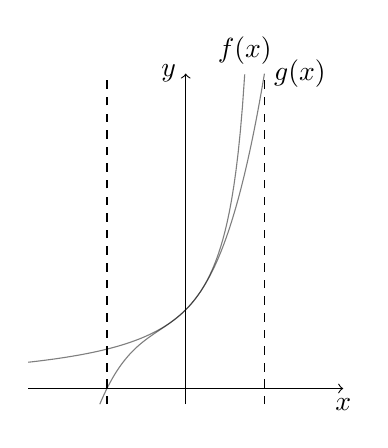
\begin{tikzpicture}[samples=100]
	\draw[->] (-2,0) to (2,0) node[below]{$ x $};
	\draw[->] (0,-0.2) to (0,4) node[left]{$ y $};

	\draw[domain=-2:0.75, opacity=0.5] plot (\x, {1/(1-\x)}) node[above,
			opacity=1]{$ f(x) $};

	\draw[domain=-1.091:1, opacity=0.5] plot (\x, {1+\x+(\x)^2+(\x)^3})
	node[right, opacity=1]{$ g(x) $};

	\draw[domain=-0.2:4, dashed] plot (1,\x);
	\draw[domain=-0.2:4, dashed] plot (-1,\x);
\end{tikzpicture}
\end{document}
